\chapter[Desenho da Aplicação]{Desenho da Aplicação}

\section{Arquitetura da Solução}

Em nossa proposta para arquitetura, podemos observar na \autoref{desenho-arquitetura} o uso de dois \textit{App Services}, onde o primeiro fará a hospedagem do \textit{front-end} da aplicação, que será desenvolvida com o \textit{framework} \textit{React}. A segunda camada fará a hospedagem de nosso \textit{Back-end} que será desenvolvida utilizando a linguagem \textit{Java}, com o \textit{framework} \textit{Springboot}.
Por fim, teremos um serviço de \textit{SQL Server}, que manterá nossas bases de dados hospedadas.

\begin{figure}[h]
\caption{Arquitetura de Solução}
\centering % para centralizarmos a figura
\label{desenho-arquitetura}

\includegraphics[width=15cm]{anexos/arquitetura_v1.png} % leia abaixo
\fonte{Os autores}
\end{figure}
\subsection{Prova de Conceito (POC)}
A \textit{Proof of Concept - POC} teve como objetivo demonstrar que o desenho de arquitetura é viável, possibilitando as integrações entre os recursos definidos e atendendo ao proposto para a aplicação.
Para isso, foram desenvolvidas duas funcionalidades simples, sendo uma de \textit{POST}, no qual poderíamos inserir um nome e endereço no \textit{front-end}, chamando a API responsável do \textit{back-end} para que realizasse a gravação dos dados no banco de dados. A segunda funcionalidade seria um \textit{GET}, onde ao realizar uma atualização na página, buscaria os dados presentes no banco de dados e exibiria no \textit{front-end}.

\subsection{Custos de mantenimento da arquitetura}
Os planos F1 dos \textit{App Services} tem gratuidade vitalícia conforme site oficial.
O plano \textit{Standard S0} para \textit{SQL Server} tem gratuidade pelos primeiros 12 (doze) meses de uso, após isso, o valor será de US\$ 14,72 (quatorze dólares e setenta e dois centavos) por mês. A \hyperlink{custos-arquitetura}{Tabela 4} mostra os valores dos recursos Azure. 

\begin{table}[h]
\hypertarget{custos-arquitetura}
	\centering\footnotesize
	\caption{\label{analise} Custos de infraestrutura da aplicação}
	%\resize
	\resizebox {0.99 \textwidth }{!}{
        \begin{tabular}{|c|c|c|c|c|c|}
        \hline
        \textbf{Serviço} & \textbf{Quantidade} & \textbf{Plano} & \textbf{Zona do serviço} & \textbf{Valor unitário} & \textbf{Total} \\ \hline
        AppService & 1 & F1 - Gratuito & East US & R\$ 0,00 & R\$ 0,00 \\ \hline
        AppService & 1 & F1 - Gratuito & East US & R\$ 0,00 & R\$ 0,00 \\ \hline
        SQL Server & 1 & Standard S0 & East US & R\$ 0,00 & R\$ 0,00 \\ \hline
        *SQL Server & 1 & Standard S0 & East US & R\$ 74,48 & R\$ 74,48 \\ \hline
        \end{tabular}
    }    
    \fonte{Os autores}
\end{table}


\section{Casos de Uso}

Os casos de uso orientam a equipe de desenvolvimento sobre o que a aplicação deverá atender. Conforme o diagrama da
\autoref{caso-de-uso}, vemos três atores principais e suas generalizações, além de suas atividades dentro da aplicação. Assim, podemos dividi-lo nos seguintes casos de uso:

\begin{figure}[h]
\caption{Casos de Uso}

\centering % para centralizarmos a figura
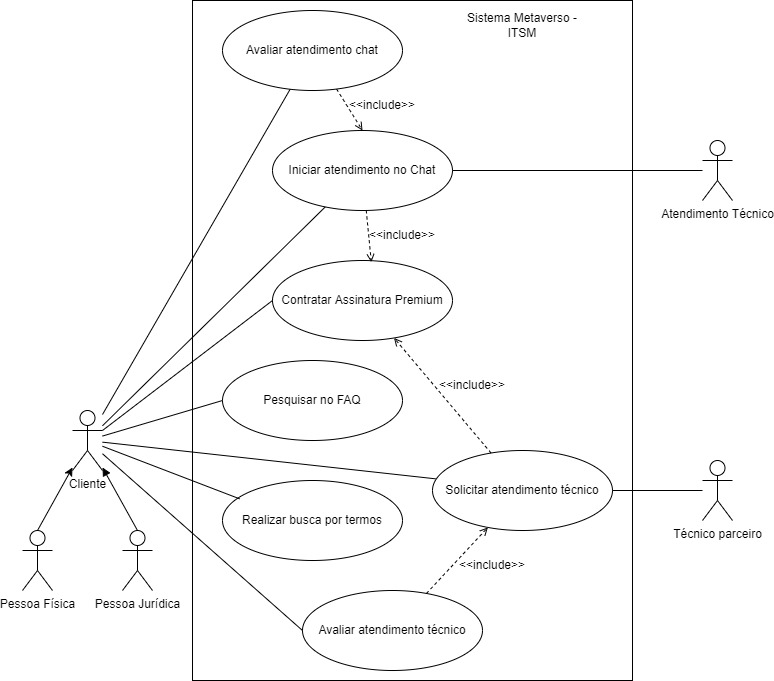
\includegraphics[width=15cm]{LaTeX/metaversoIFSP/anexos/Casos de Uso.jpeg} % leia abaixo
\label{caso-de-uso}
\fonte{Os Autores}
\end{figure}

\subsection{Caso de Uso: Contratar Assinatura \textit{Premium}}
O cliente, que pode ser pessoa física ou jurídica, se torna um assinante \textit{Premium} da aplicação, mediante pagamento mensal de um valor pré-determinado, de acordo com o plano contratado. Alguns dos próximos casos de uso estão vinculados ao usuário ter a assinatura ativa para conseguir utilizar.

\subsection{Caso de Uso: Pesquisar no FAQ}
O cliente navega dentro do FAQ, visualizando categorias que levem-o até o problema que o mesmo tenha e disponibilize uma solução.

\subsection{Caso de Uso: Realizar busca por termos}
O cliente poderá, após a pesquisa no FAQ sem sucesso, realizar uma busca dentro da própria aplicação através de poucas palavras que poderá indicar links de outros sites e fóruns potencialmente úteis para solucionar seu problema.

\subsection{Caso de Uso: Iniciar atendimento no \textit{Chat}}
O cliente poderá a qualquer momento, desde que seja um assinante Premium ativo, iniciar um atendimento técnico via chat, onde terá auxílio para resolver os problemas técnicos de seu dispositivo.

\subsection{Caso de Uso: Avaliar atendimento \textit{Chat}}
O cliente que tiver passado por um atendimento via \textit{chat}, conforme mencionado no caso anterior, poderá avaliar o atendimento, contribuindo para a melhoria da aplicação e parceiros.

\subsection{Caso de Uso: Solicitar atendimento técnico}
O cliente pode solicitar um atendimento técnico, que poderá ser multicanal (telefone, mensagens, remota ou presencial) de um técnico parceiro. A ferramenta listará os técnicos da região disponíveis para atender o chamado de acordo com sua especialidade, onde o cliente pode escolher o técnico ou deixar em aberto para que os técnicos possam aplicar para atender o atendimento.

\subsection{Caso de Uso: Avaliar o atendimento técnico}
O cliente que tiver solicitado atendimento técnico avalia o mesmo, contribuindo para a relevância do técnico parceiro dentro da ferramenta e para possíveis melhorias dentro da plataforma.
\section{Regras de Negócio}
As regras de negócio são descritas na \hyperlink{tabela-regra-negocio}{Tabela 5}.

\begin{table}[h]
\hypertarget{tabela-regra-negocio}
	\centering\footnotesize
	\caption{Regras de negócio}
	\resizebox {.8 \textwidth }{!}{
        \begin{tabular}{|l|p{8cm}|}
        \hline
        \textbf{Identificador}            & \textbf{Regra de negócio}                                                         \\ \hline
        RN01 & O cliente que é assinante poderá ir diretamente ao chat de atendimento técnico para resolver seu problema                      \\ \hline
        RN02 & Caso o cliente é assinante e não encontrou a solução do seu problema via FAQ, o cliente assinante poderá acessar ao chat de atendimento                   \\ \hline
        RN03 & O cliente assinante entra em contato via chat, mas não consegue resolver seu problema. Então, poderá realizar o agendamento a uma visita técnica                   \\ \hline
        RN04 & Caso o técnico não consiga realizar o reparo/manutenção, será agendado para outro técnico                  \\ \hline
        RN05 & O usuário que acessa a plataforma de forma gratuita só poderá navegar pelos FAQs.                  \\ \hline
        \end{tabular}
    }    
\end{table}
\fonte{Os autores}
\newpage
\section{Requisitos Funcionais}
Os requisitos funcionais são descritos na \hyperlink{tabela-requisitos-funcionais}{Tabela 6}.

\begin{table}[h]
\hypertarget{tabela-requisitos-funcionais}
	\centering\footnotesize
	\caption{Requisitos Funcionais}
	\resizebox {1.0 \textwidth }{!}{
        \begin{tabular}{|l|p{8cm}|p{8cm}|}
        \hline
        \textbf{Identificador}            & \textbf{Requisito} & \textbf{Descrição}                                                            \\ \hline
        RF01 & O sistema deve permitir o cadastro de técnicos  & O sistema deve permitir que técnicos consigam realizar o cadastro para adicionar os dados de identificação                        \\ \hline
        RF02 & O sistema deve permitir cadastro de clientes facilitada  & O sistema deve permitir que clientes consigam realizar o cadastro com o mínimo de dados necessários e, posteriormente, incluir dados adicionais                       \\ \hline
        RF03 & O sistema deve permitir abertura de chamado  & O cliente deve conseguir detalhar o problema que não conseguiram resolver pelo FAQ             \\ \hline
        RF04 & O sistema deve permitir a visualização de histórico do chamado  & O usuário poderá acompanhar histórico de seus chamados, andamento e avaliações           \\ \hline
        RF05 & O sistema deve permitir cadastro de instruções no FAQ  & O sistema deve permitir que novas soluções sejam criadas, editadas, suprimidas ou deletadas no FAQ \\ \hline
        RF06 & O sistema deve permitir a realização do login  & O sistema deve permitir a realização do login para os usuários que estão cadastrados na plataforma \\ \hline
        RF07 & O sistema deve permitir visualização de histórico de incidentes  & O sistema deve permitir que técnicos tenham a visualização ao histórico de problemas e tratativas que foram aplicadas para um cliente ao realizar um atendimento 		\\ \hline
        \end{tabular}
    }    
\end{table}
\fonte{Os autores}
\section{Requisitos Não Funcionais}
Os requisitos não funcionais são descritos na \hyperlink{tabela-requisitos-nao-funcionais}{Tabela 7}.

\begin{table}[h]
\hypertarget{tabela-requisitos-nao-funcionais}
	\centering\footnotesize
	\caption{Requisitos Não Funcionais}
	\resizebox {1.0 \textwidth }{!}{
        \begin{tabular}{|l|p{14cm}|c|}
        \hline
        \textbf{Identificador}            & \textbf{Requisitos}       & \textbf{Categoria}                                           \\ \hline
        RNF01 & O usuário não deve demorar mais que 10 segundos para identificar a seção relevante para sua busca &   Usabilidade           \\ \hline
        RNF02 & O sistema deve respeitar a LGPD      & Segurança                \\ \hline
        \end{tabular}
    }    
\end{table}
\fonte{Os autores}
\section{MER e DER}
Os diagramas representados nos mostram a estrutura de tratamento de dados e processos dos usuários, conforme \autoref{mer-usuario} e \autoref{der-usuario}, assim como as tabelas para gerenciamento de nosso serviço do FAQ, vide \autoref{der-faq} e \autoref{mer-faq}.

\begin{landscape}
\begin{figure}[h]
    \caption{Modelo conceitual - Usuários e seus relacionamentos}
    
    \centering % para centralizarmos a figura
    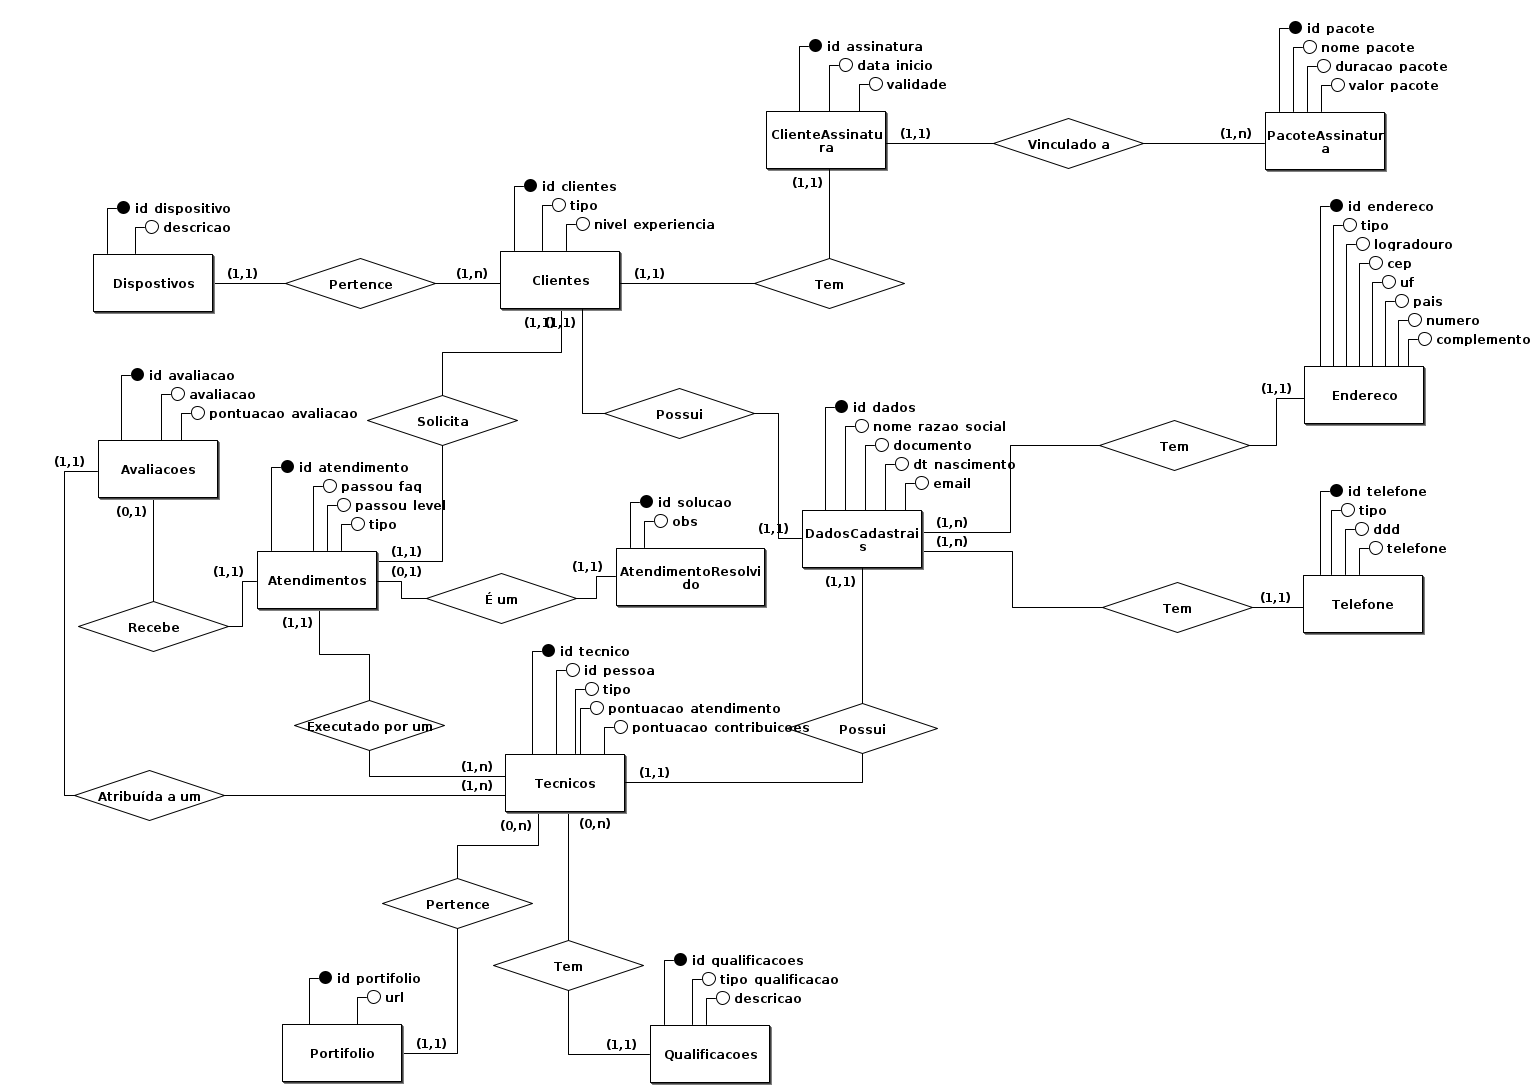
\includegraphics[width=19cm]{LaTeX/metaversoIFSP/anexos/MER-Usuarios.png} % leia abaixo
    \label{mer-usuario}
    \fonte{Os Autores}
\end{figure}

\end{landscape}
\begin{landscape}
\begin{figure}[h]
    \caption{Diagrama Entidade-Relacionamento - Usuários e seus relacionamentos}
    
    \centering % para centralizarmos a figura
    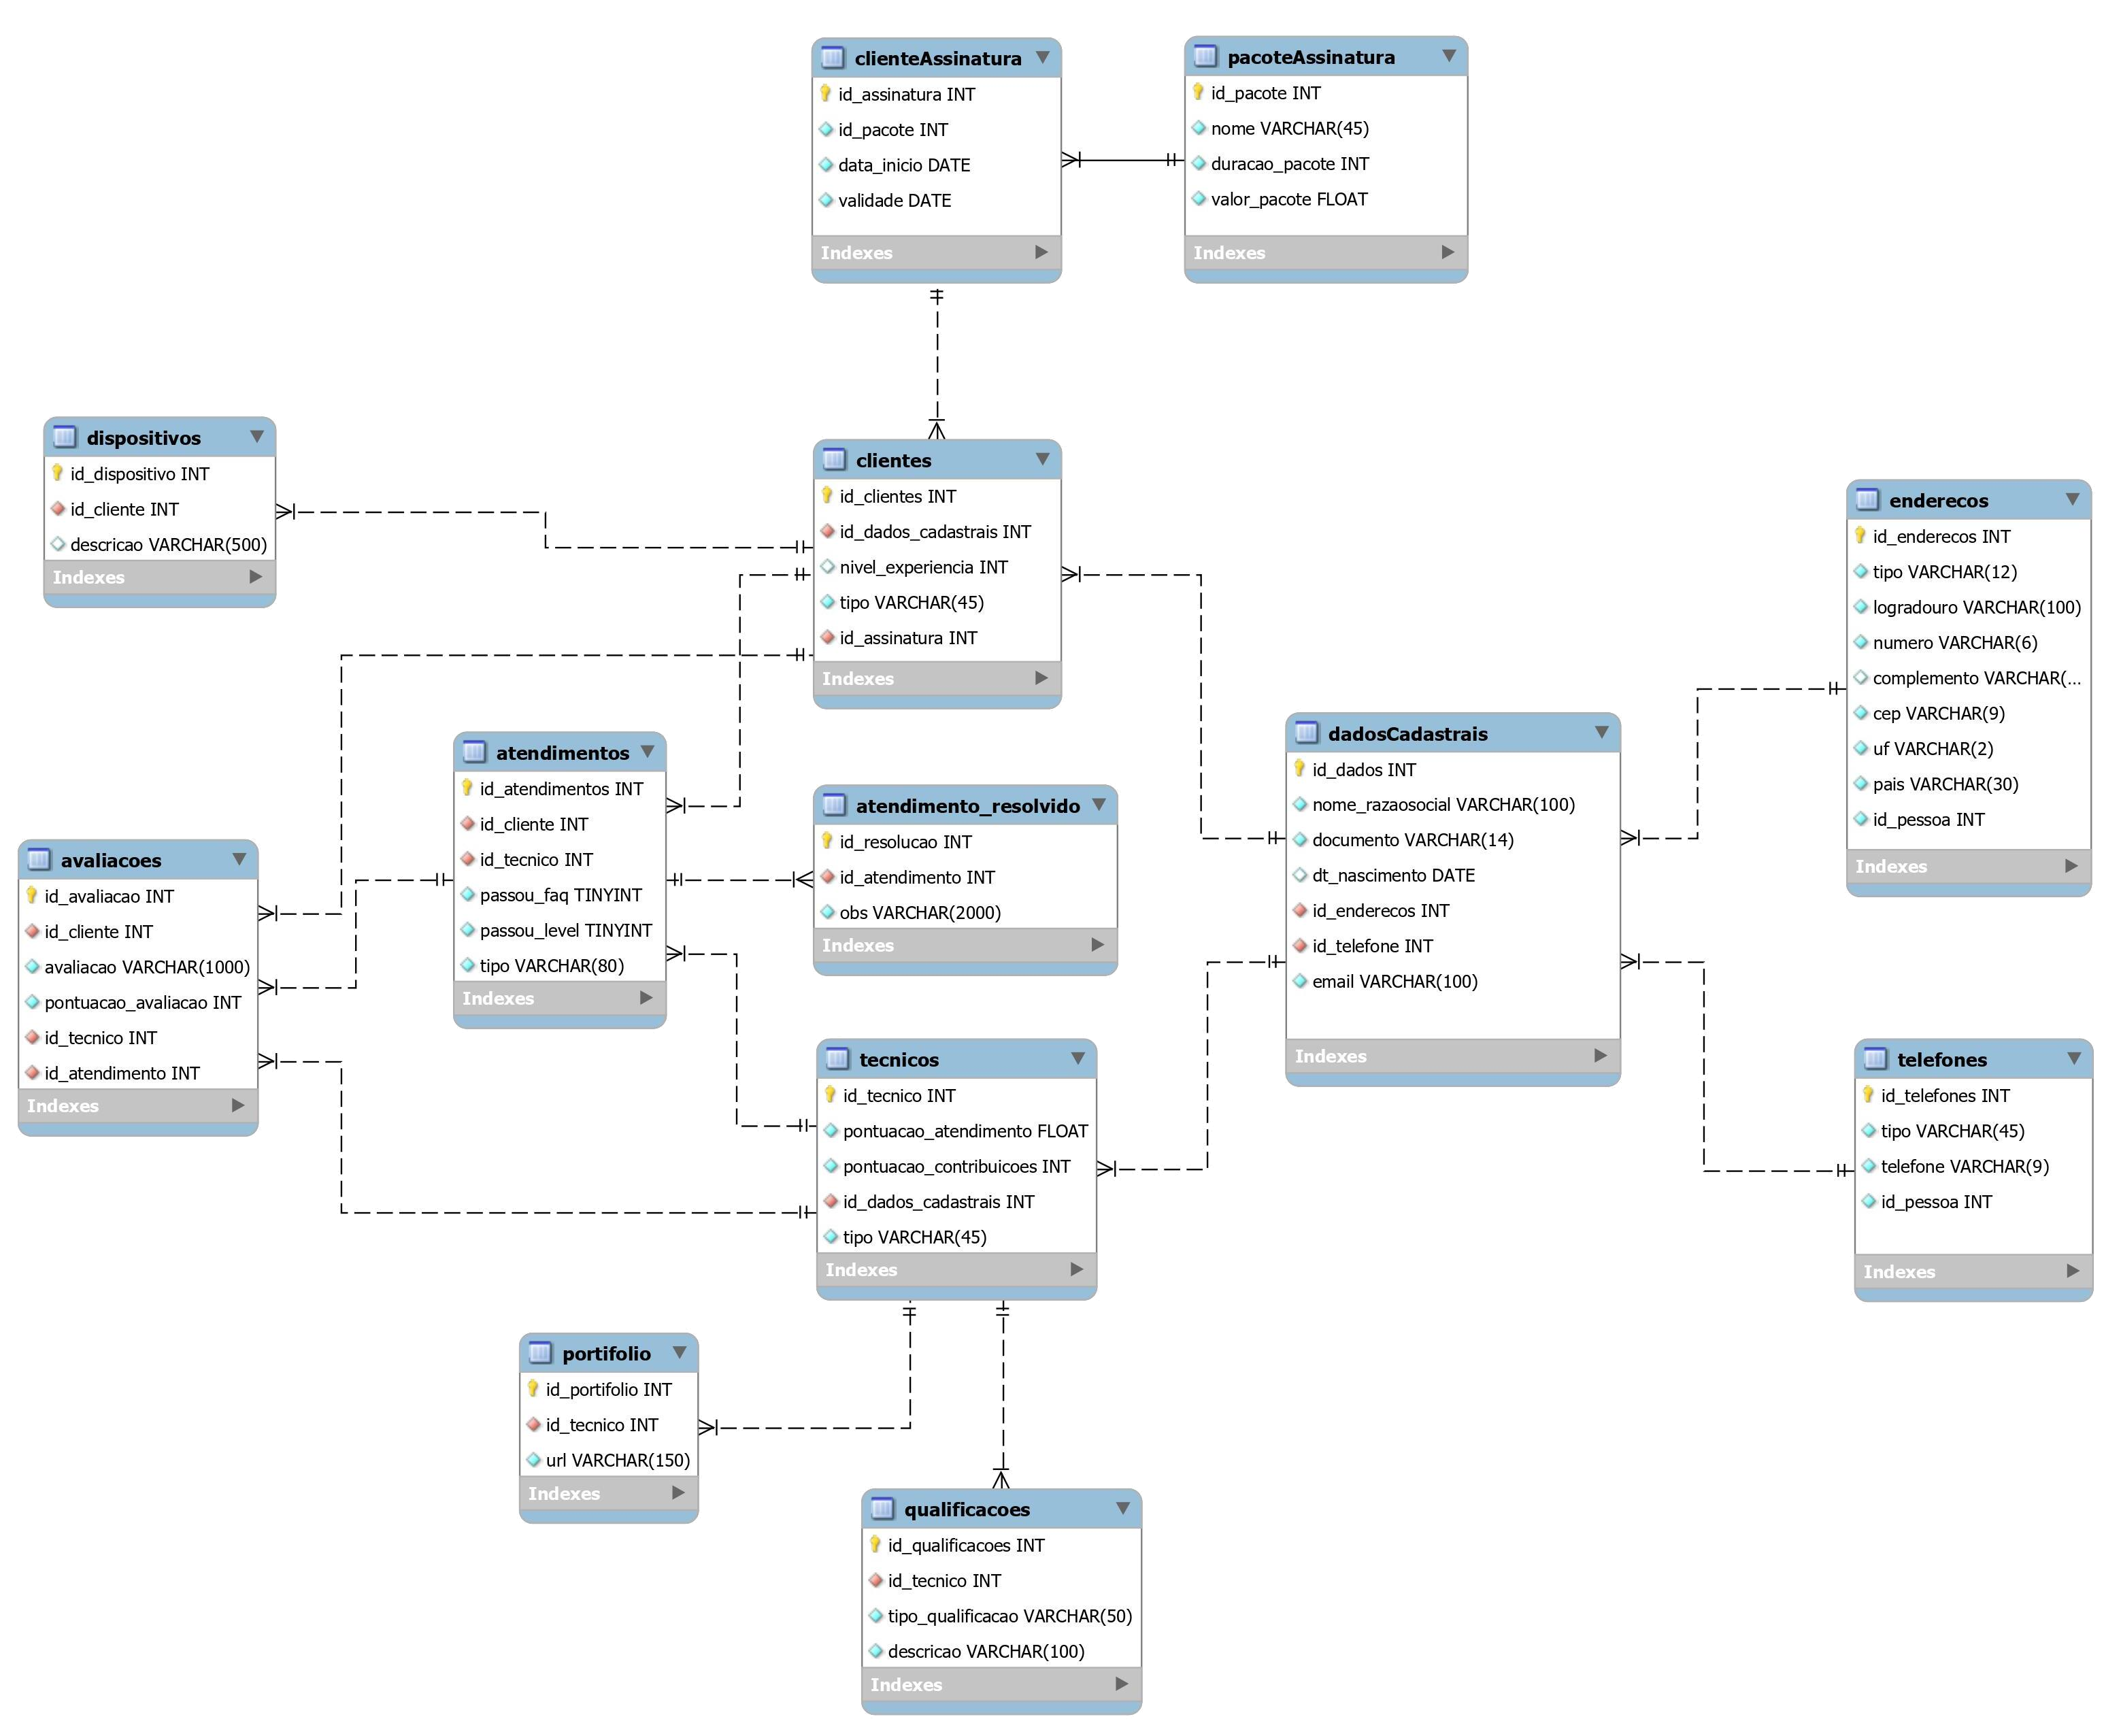
\includegraphics[width=19cm]{LaTeX/metaversoIFSP/anexos/DER-Usuarios-e-Derivados.png} % leia abaixo
    \label{der-usuario}
    \fonte{Os Autores}
\end{figure}
\end{landscape}

\begin{landscape}
    \begin{figure}[h]
        \caption{Diagrama Entidade Relacionamento - \textit{FAQ}}
        
        \centering % para centralizarmos a figura
        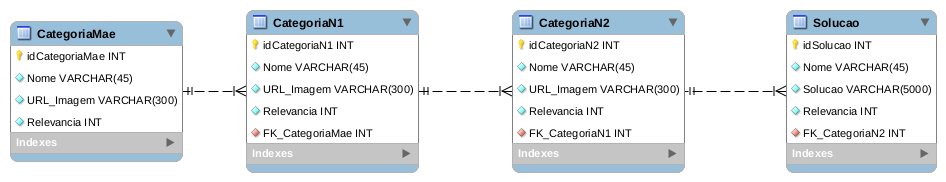
\includegraphics[width=23cm]{LaTeX/metaversoIFSP/anexos/DER-FAQ.png} % leia abaixo
        \label{der-faq}
        \fonte{Os Autores}
    \end{figure}
    
    \begin{figure}[h]
        \caption{Modelo Conceitual - \textit{FAQ}}
        
        \centering % para centralizarmos a figura
        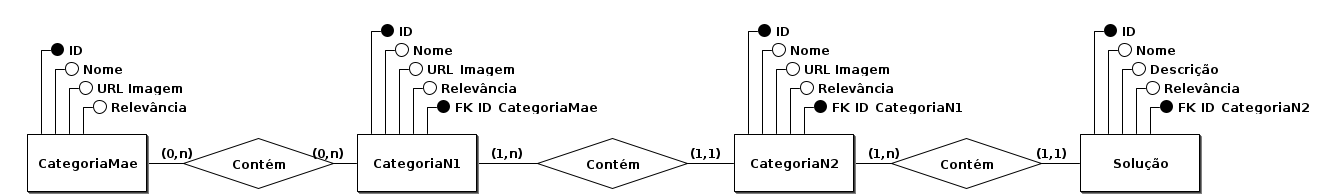
\includegraphics[width=23cm]{LaTeX/metaversoIFSP/anexos/FAQ-Conceitual.png} % leia abaixo
        \label{mer-faq}
        \fonte{Os Autores}
    \end{figure}
\end{landscape}

 
%\section{Justificativa}
%\section{Estrutura do Estudo}

%\lipsum[3-5]
%Teste de citação para gerar referências no modelo.. \citeauthor{SCRUMGUIDE:2013}

% ----------------------------------------------------------
% Referências bibliográficas
% ----------------------------------------------------------
%\bibliography{referencias,exemplos/abntex2-doc-abnt-6023}
